\section{Durchführung}
\label{sec:Durchführung}

Die in diesem Versuch verwendete Messapparatur ist in Abbildung \ref{fig:aufbau}
dargestellt.

\begin{figure}[H]
  \centering
  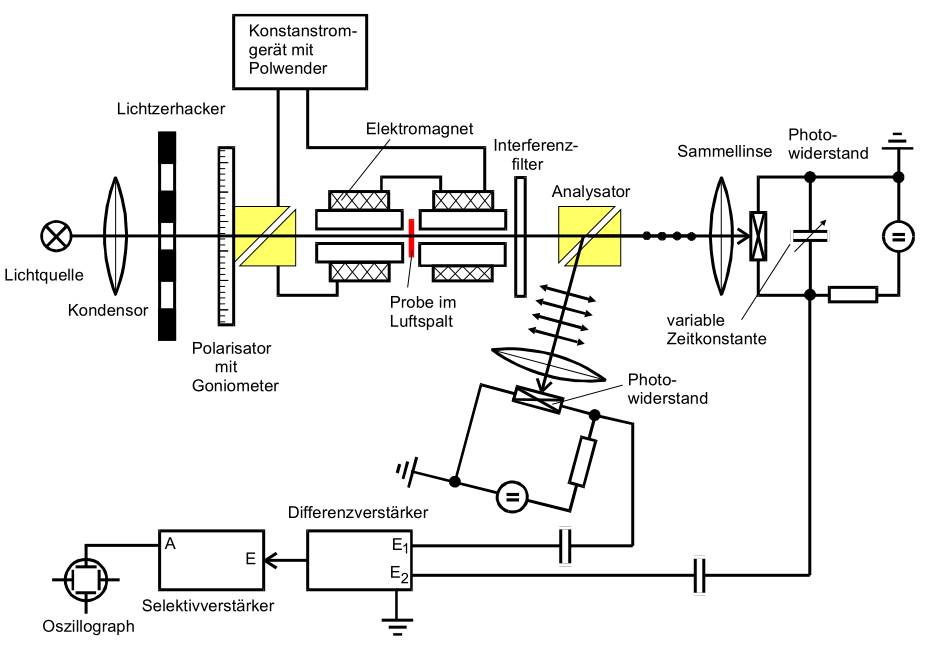
\includegraphics[height=10cm]{Aufbau.PNG}
  \caption{Schematische Darstellung des Versuchsaufbaus. \cite{sample}}
  \label{fig:aufbau}
\end{figure}

Als Lichtquelle dient eine Halogenlampe das emittierte Licht wird über eine
Kondensorlinse gebündelt und fällt dann durch rotierendes Rad, welches als Lichtzerhacker
dient. Dadurch wird der kontinuierliche Lichtstrahl in einzelne Lichtimpulse unterteilt.
Anschließend fällt das Licht auf einen Polarisator. Dabei handelt es sich um
ein sogenanntes Glan-Thomson Prisma (Abbildung \ref{fig:prisma}). Aufgrund der doppelbrechenden Eigenschaften
des Materials, aus welchem das Prisma besteht, wird das einfallende Licht in
zwei senkrecht zueinander linear polarisierte Lichtstrahlen aufgeteilt (ordentlicher Strahl
und außerordentlicher Strahl). Das Prisma ist dann schräg in der Mitte geteilt,
sodass sich ein kleiner Spalt Luft zwischen den beiden Elementen befindet.
An der Grenzfläche Kristall - Luft wird einer der beiden Strahlen dann totalreflektiert,
wodurch sich in die ursprüngliche Ausbreitungsrichtung nur noch ein linear polarisierter
Lichtstrahl ergibt.

\begin{figure}[H]
  \centering
  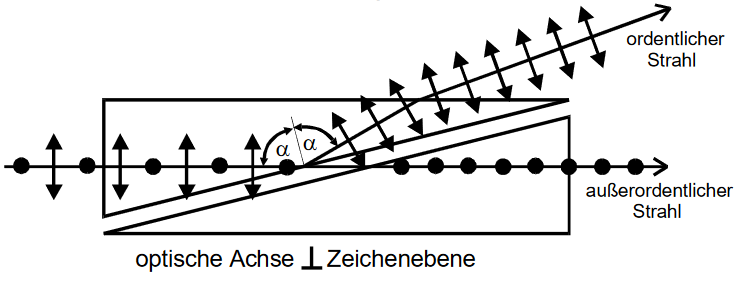
\includegraphics[height=5cm]{Prisma.PNG}
  \caption{Schematische Darstellung eines Glan-Thomson Prismas. \cite{sample1}}
  \label{fig:prisma}
\end{figure}

Hinter dem Polarisator befindet sich dann letztendlich die Probe, welche sich im Einflussgebiet
eines darum befindlichen Elektromagneten befindet. Es folgt ein Interferenzfilter (Abbildung \ref{fig:filter}),
mit dessen Hilfe nur jeweils eine bestimmte Wellenlänge des Lichts herausgefiltert
wird. Er besteht aus einer dünnen Schicht eines transparenten Dielektrikums, welches
von zwei semitransparenten Schichten umgeben ist. Durch Reflexion an diesen Schichten
interferieren sich alle Anteile des Lichtes heraus, welche nicht die durch die Geometrie
des Filters gegebene Interferenzbedingung erfüllen.

\begin{figure}[H]
  \centering
  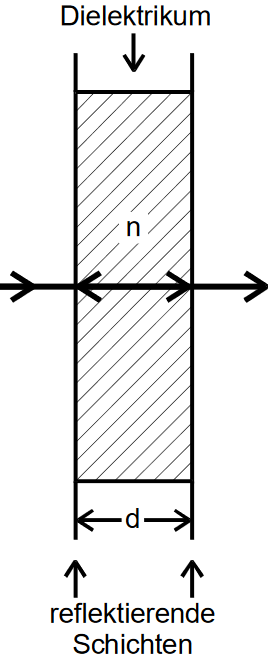
\includegraphics[height=8cm]{Interferenzfilter.PNG}
  \caption{Schematische Darstellung eines Interferenzfilters. \cite{sample1}}
  \label{fig:filter}
\end{figure}

Hinter dem Interferenzfilter befindet sich dann ein weiteres Glan-Thomson Prisma,
welches hier jedoch als Analysator genutzt wird. Wie oben beschrieben, treten zwei
senkrecht zueinander polarisierte Lichtstrahlen aus dem Prisma heraus, welche letztendlich
durch zwei Photowiderstände gemessen werden. Die gemessenen Spannungen an den Photowiderständen
werden auf einen Differenzverstärker gegeben. Dieser liefert als Signal das Ergebnis der voneinander
abgezogenen Intensitäten der einzelnen Widerstände. Es folgt noch ein Selektivverstärker, welcher
lediglich das Signal in einem Bereich um die Frequenz der Lichtzerhackers verstärkt, um
zusätzlich Störspannung herauszufiltern. Das Signal wird letztendlich auf
ein Oszilloskop gegeben. Der Drehwinkel der Polarisationsebene des linear polarisierten Lichts
kann nun bestimmt werden, indem das Signal des Differenzverstärkers durch Drehung des
Polarisationsprismas auf sein Minimum abgeregelt und der entsprechende Winkel gemessen
wird. Sodann wird das Magnetfeld des Elektromagneten umgepolt und erneut der
Winkel des nun entstandenen Minimums gemessen. Aus diesen Werten lässt sich dann der
jeweilige Ablenkwinkel nach
\begin{equation}
  \Theta  = \frac{1}{2} \cdot (\Theta_r - \Theta_l)
\label{eqn:drehwinkel}
\end{equation}
bestimmen.

Auf eben diese Weise werden im Versuch dann zwei dotierte, sowie eine hochreine
GaAs-Probe untersucht. Dazu werden die entsprechenden Winkel für verschiedene
Wellenlängen (also unterschiedliche Interferenzfilter) gemessen.

Schließlich wird dann noch mit einer Hallsonde die Stärke des Magnetfeldes an der
Stelle der Probe gemessen.
